\documentclass[twocolumn, 10pt]{article}
\usepackage{geometry}                % See geometry.pdf to learn the layout options. There are lots.
\geometry{letterpaper}                   % ... or a4paper or a5paper or ... 
\usepackage[parfill]{parskip}    % Activate to begin paragraphs with an empty line rather than an indent
\usepackage{graphicx}
\usepackage{amssymb, amsmath}
\usepackage{fullpage}

\usepackage{fourier}
\usepackage{courier}

\setcounter{secnumdepth}{0} % supresss section numbers

% Nice captions.
\usepackage[hang,small,bf]{caption}
\setlength{\captionmargin}{25pt}

\title{Aggregation Optimizations for Skewed Data}
\author{Josh Rosen}

\newcommand{\keyspace}{\mathcal{K}}


\begin{document}
\maketitle

\section{Introduction}

Aggregate-by-key is a common (and often expensive) operation in ``big data''
frameworks like MapReduce and Spark.
%
There are many ways to optimize aggregation, including multi-level
aggregation techniques, like aggregation trees, and pre-aggregation
techniques, like Hadoop and Spark's map-side combiners.

As a framework for analyzing these optimizations, we can view aggregators as
functions whose output key distributions are ``flattened'' versions of their
input key distributions.  The degree of this flattening depends on the aggregation
technique and properties of the input data, such as clusteredness or skew.

For example, a buffering aggregator with unlimited buffer space produces
uniform output key distribution for any input distribution.  A pre-aggregator
with finite buffer space may leave the key distribution untouched in the worst
case, or may achieve perfect flattening in the best case.

\subsection{Analysis Framework}

In our framework, an aggregator is a stateful operator that receives an input
stream of (key, value) pairs and produces an output stream of (key, aggregate)
pairs.  Let each input key $k$ be randomly sampled with replacement
from a discrete distribution $p_{in}(k)$ defined over a finite keyspace
$\keyspace$.  The aggregator's behavior defines
a distribution of output sizes and output key distributions $p_{out}(k)$.
The output key distribution is guaranteed to be at least as uniform as the
input distribution.

\begin{figure*}
\begin{center}
    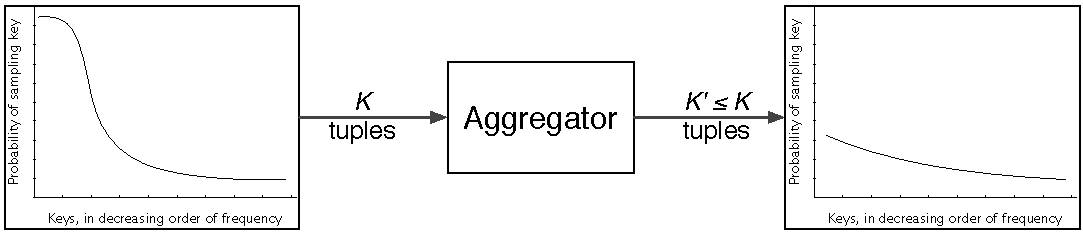
\includegraphics[width=0.8\textwidth]{figures/aggregator_as_filter}
\end{center}
\caption{Aggregators can be viewed as stream filters that perform lossless
compression by removing skew.}
\label{fig:aggregator_as_filter}
\end{figure*}

As an example, an aggregator with unlimited buffer space produces output whose
size is equal to the number of distinct keys in its input and whose key
distribution is uniform.

Because the inputs and outputs of aggregators are both modeled as key
frequency and output size distributions, we can use conditional probability to
analyze the composition of two aggregators.  For example,
Figure~\ref{fig:aggregator_pipeline} shows a network of pipelined aggregators.
To analyze the output distribution of the pre-aggregator, we can consider the
fact that its input tuples have hit the Bloom filter (more generally, we could
have filters that route inputs based on predicates).

Even though we are modeling distributed aggregate-by-key, our analysis will
only focus on the final output produced by a particular reducer.  Reducers
operate on disjoint sets of keys; if we assume that all reducers are
responsible for the same number of distinct keys (a reasonable assumption when
using hash-partitioning), then we can model the complete aggregation
by combining the independent analyses of the individual reducers.

\section{Pre-Aggregation}

In engines like MapReduce, aggregation queries can be executed by
shuffling the dataset based on its grouping attribute(s), then applying a local
aggregation algorithm on each post-shuffle group.
This final aggregation can be performed using hash- or sort-based algorithms
(or hybrids of the two, as in \cite{aggregation-revisited}).

This can be optimized using \emph{pre-aggregation}, where the aggregation is
performed in two phases: first, each mapper performs a local aggregation
of its data; next, these aggregates are shuffled and a final aggregation is
performed on each group.
This corresponds to Hadoop's ``Combiners'' feature.
For this optimization to apply, the aggregation function has to be commutative
and associative.
% TODO: is this strictly true, or can we use a more-precise or weaker set of properties?

Pre-aggregation can improve performance by reducing the volume of data set
over the network and by distributing the CPU cost of applying the aggregation
function to popular keys.
These benefits come at the cost of additional work during the pre-shuffle phase.

The performance of aggregation algorithms is affected by the number of groups.
Map-side pre-aggregation may have to aggregate up to $|\keyspace|$ groups,
but, assuming a reasonable key partitioning function, the $r$ reduce-side final
aggregators only need to aggregate up to $|\keyspace|/r$ groups.  In many cases,
the number of groups may be too large to efficiently perform complete
pre-aggregation.

Because the output of pre-aggregators undergoes a final post-shuffle
aggregation, we can apply \emph{partial pre-aggregation}
\cite{partial-preaggregation}, where we allow mappers to produce multiple
partial aggregates for a given group.  Partial pre-aggregation
is a nonblocking operator, allowing the pre-aggregation and shuffle phases
to be pipelined.

Partial pre-aggregators can operate with limited amounts of memory, since in the
worst case they could perform no aggregation.  With a hash-based
pre-aggregator, incoming values can be aggregated into matching entries in the
hashtable or inserted as new entries.  When the hashtable becomes full, the
aggregator can use an \emph{eviction strategy} to free up space.
Some simple eviction strategies include LRU, randomized eviction, or complete
emptying of the hashtable whenever it becomes full.
Values can be evicted by spooling them to disk or, in the pipelined case, by
sending them across the network to their final aggregator.
The pre-aggregator could also decide to bypass the per-aggregation for some
incoming tuples by immediately spooling or sending them.

Eviction and bypass strategies have been studied extensively in caching; many
of the techniques that we'll explore have their origins in web caching or CPU
cache mechanisms.  The pre-aggregation setting is slightly different
in the sense that the marginal cost of an individual cache miss is small.  In
processor caches, a cache miss may be orders of magnitude more expensive than
a hit, while here we only pay the cost of shuffling one additional tuple.
However, these costs can add up quickly if a frequent key isn't cached.

\subsection{Analysis of Partial Pre-Aggregators}

We want to analyze hash-based pre-aggregators by estimating their output size
and distribution given an input distribution.  Pre-aggregators' performance is
sensitive to input orderings.  In the best case, the input is perfectly
clustered by key (all occurrences of a key appear back-to-back) and only one
unit of buffer space is needed to achieve an optimal pre-aggregation.  In the
worst case, the input could maximize the interarrival times of all keys,
leading to high hashtable churn.  For now, we'll ignore these effects and
assume that the input arrives in a random order where keys' interarrival rates
are based on their frequencies in the input distribution.

We'll also ignore boundary conditions, such as when the hashtable is initially
empty or when all keys are flushed at the end of the job, by assuming that
our input stream is infinite and analyzing the ``steady-state'' condition where
the hashtable is always full.


%This is exactly analagous to cache eviction policies, where we want to maximize cache hits (preaggregations), and algorithms like LRU or LFU can be used.
%The optimal eviction strategy is to evict the key that will be hit furthest in
%the future \cite{Belady1966}; it's not possible to actually implement this
%strategy, but it provides an upper bound on the effectiveness of our eviction
%strategy.

%\subsection{Pre-aggregation and Skew}

%Skew can affect pre-aggregation's cost and benefit.  Key-value pairs can exhibit both input and output skew \cite{adaptive-aggregation}.
%With \emph{input skew}, all nodes have the same number of groups but different numbers of records.  Input skew can cause a particular node to become a straggler because it has more input data to process.  In contrast, with \emph{output skew}, nodes have the same number of records but different numbers of groups or distinct keys, which means that some nodes may not have enough buffer space to pre-aggregate all groups.

%\subsection{When to Apply Pre-aggregation}

%To decide whether to apply total pre-aggregation or to shuffle the entire
%dataset, we can calculate the total number of groups being aggregated, since
%pre-aggregation is beneficial when there are relatively few keys, but may harm
%performance on data sets with huge numbers of unique or infrequent keys
%\cite{adaptive-aggregation}.
%Sampling techniques can be used to estimate the number of groups.
%Some systems pick an initial aggregation strategy and adaptively change it if
%the original cost estimates appear to be wrong (e.g. by having nodes
%autonomously switch from total pre-aggregation to direct shuffling of tuples
%if they do not have enough buffer space for the pre-aggregation hashtable)
%\cite{adaptive-aggregation}.
%
%Partial pre-aggregation is sensitive to the input data ordering, complicating
%this trade-off.  If the input is perfectly clustered by the grouping
%attributes, then pre-aggregation requires one partial results' worth of buffer
%space to achieve the maximum reduction in output size.  Knowing the exact
%distribution of values across groups doesn't help here, since an adversarial
%input ordering can lead to high eviction rates.



%%%%%%%%%%%%%%%%%%%%%%%%%%%%%%%%%%%%%%%%%%%%%%%%%%%%%%%%%%%%%%%%%%%%%%%%%%%%%%
\section{Bloom Filter Cache Bypassing}

If a key appears only once in an input stream (or rarely, with very high
interarrival times), it can't benefit from pre-aggregation.  If an aggregator
could identify these keys, it could forward them immediately rather than
futilely buffering them. 

The challenge is in identifying unique keys while using a minimal amount of
space, since skewed datasets may have large ``long tails'' of unique keys.
Bloom filters can help here: if we look up all incoming keys in
a Bloom filter, we can bypass the pre-aggregation for the first occurrence of
any key.  This approach has two limitations: false-positives may cause
a unique key to be pre-aggregated, and we may need a large Bloom filter to
achieve a low false positive rate when processing a dataset with many unique
keys.

To address these limitations, we can consider using a small Bloom filter that's
periodically cleared once a certain fraction of its bits are set (or,
equivalently, when the expected false positive probability exceeds some
threshold).  For unique keys, this approach will lower the false positive
probability, but it may lead to false negatives for non-unique keys.
We can avoid those false negatives by re-inserting the aggregation buffer's
keys into the Bloom filter after clearing it.

Informally, we can see that this is beneficial by considering pre-aggregation
over an infinite stream with an infinite number of unique keys and an infinite
number of reappearances of non-unique keys.  A finite Bloom filter will
eventually fill up and become useless due to the infinite number of unique
keys, while periodically clearing it avoids this.

A similar approach has been proposed for processor caches
\cite{evicted-address-filter}, using a Bloom filter to construct an
\emph{evicted address filter} to identify memory addresses that miss the cache
multiple times within a short time window; this allows the cache to
distinguish between high-reuse and low-reuse blocks when deciding which blocks
to cache, helping to avoid cache pollution and thrashing.
% TODO: the above paper has more details.

% TODO: discuss appropriate sizing of the Bloom filter as a function of the
% cache size.


\subsection{Analysis of Bloom Filter Cache Bypassing}

For an infinite input stream, we'd like to determine the size and frequency
distributions for the sets of keys that hit the Bloom filter and the keys that
miss it.


%Again, we're faced with a trade-off: if we maintain a list of records with poor hit ratios, the space used to maintain that list could also be used to have a bigger cache.  In processors, you can classify individual instructions in a loop as ``tends to cause cache misses`` (or hits), so you only need a small dense array to track hit rate information \cite{automatic-cache-bypass}.

% TODO: a large portion of the literature here seems to be in patents.

% It looks like a relevant search term is "adaptive cache manamgement strategies"

% TODO: parallelism: can you pipeline this process, having one thread sort pages of records at a time while another thread consumes sorted pages and probes the hashtable?

% TODO: what about associativity?










%%%%%%%%%%%%%%%%%%%%%%%%%%%%%%%%%%%%%%%%%%%%%%%%%%%%%%%%%%%%%%%%%%%%%%%%%%%%%%



\section{Multi-level Aggregation}

Multi-level aggregation techniques, such aggregation trees, can address
several problems:

\begin{itemize}
    \item In wireless sensor networks, the network may not be fully-connected
    and some pairs of nodes must communicate through other intermediate nodes.
    To save bandwidth (which can lead to large power savings), aggregation can
    be performed at intermediate nodes of the spanning tree \cite{tag}.

    \item Even if all pairs of nodes can directly communicate, the underlying
    network topology may not be flat: for example, intra-rack bandwidth can be
    much greater than inter-rack bandwidth.  In these cases, aggregation trees
    can reduce the amount of data communicated through the cross-rack
    bottleneck.

    \item A node's bandwidth is usually shared by all parties communicating
    with it, so aggregation schemes that send all data to a single node may
    become bottlenecked on that machine's individual network link; aggregation
    trees can alleviate this problem by reducing the total amount of data sent
    to any individual machine.
    % TODO: a comment on MPI-style AllReduce might be appropriate somewhere.

    \item For popular keys, aggregation trees can distribute the processing
    cost of applying the aggregate function.

\end{itemize}

Hierarchical aggregation consumes more total resources than flat aggregation
but allows parallelism to be exploited.  If the aggregation can be parallelized
such that each aggregator makes progress by producing output that's smaller
than its combined inputs, then hierarchical aggregation can be beneficial.
If the individual aggregators achieve little or no reduction of their inputs,
then hierarchical aggregation may harm performance (for example, an
aggregation tree could cause a logarithmic increase in execution time for
inputs that don't benefit from it).

% TODO: this bit about "logarithmic increase" is confusingly-worded.

% Note: the above bit about "more total resources" may depend on how we're
% billed for those resources.  Per-operation billing is different than
% per-second-of-wallclock-time-irrespective-of-utilization.

For some inputs, it's clear whether aggregation trees will be beneficial.
For dense numeric vectors, an aggregator with $f$ inputs produces output
that's $1/f$ of its input size, achieving the maximum possible reduction.
For the opposite case, imagine aggregating a set of sparse vectors with
no common non-zero entries; in this case, aggregators perform no reduction of
their input.

In general, sparse vectors occupy a space between these two extremes: the
degree of sparsity and skew determines whether aggregation trees are
beneficial.  We can view sparse vectors as sets of (index, value) pairs, so we
can analyze this problem using our aggregate-by-key framework.

\subsection{Analysis of Aggregation Trees}

Given $m$ machines each producing $K$ keys, what's the optimal fan-in for an
aggregation tree that produces a final aggregate at its root?  The maximum
fan-in, $m$, is equivalent to sending all keys to the root.  The minimum
fan-in, 2, produces a binary aggregation tree.

Assume that the leaves of the aggregation tree perform no local combining.
If our goal is to minimize communication, $m$ is the optimal fan-in.
Minimizing the total time to produce the final aggregate is more complicated.
The end-to-end time is determined by the sum of the maximum completion times
at each level of the aggregation tree.  Let $|a_{out}|$ be the number of
records output by aggregator $a$.  If we assume that the network behaves
linearly and each aggregator spends one unit of processing and communication
time per input record, then with a fan-in of $f$ the end-to-end time is
\[
    \sum_{l=1}^{\lceil\log_fm\rceil}
        \max
        \left(
            |a_{out}| | a \in \text{ level } l
        \right)
\]
If aggregators perform complete aggregation over their inputs, their output
size is the number of unique keys in their inputs.

When the dataset contains only one key, a fan-in of $f$ produces a tree
where each level takes $f$ units of time to complete, for a total time of
\[
    f \log_f m,
\]
which is minimized by $f = e$.  Since $f$ must be discrete, the optimal fan-in
is $f = 3$, because $3 \log_3 m \leq 2 \log_2 m$ for $m > 1$.

In a more general case, the input dataset could be a sample of $m$ random
$K$-subsets of the keyspace (of size $|\keyspace|$) where we have some
probability distribution over subsets.  Alternatively, we could imagine the
input as $m$ random $K$-samples without replacement from the keyspace given
a probability distribution over keys.

To estimate the end-to-end time for an $f$-ary aggregation, we must
estimate the sum of the maximum input sizes for leaves at each level of the
tree.  For any subtree, the root's input size is equal to the number of
distinct keys present at the leaves of that subtree.  Thus, the probability
that the root of the aggregation tree receives $x$ keys as input is equal to
the probability that the $m$ leaves have $x$ distinct keys in common.

There are results for estimating the size of the union of equal-size subsets
of a set \cite{union-of-subsets}, but unfortunately there aren't results for
the union of different arbitray-sized subsets.
% http://www.pnas.org/content/109/19/E1183.full#xref-ref-38-1 says that
% this appears to be an open problem, as of 2012.
To work around this, we can treat subtrees as independent and work with
expected values (subtrees are dependent because their input sizes are
conditionally dependent on their parent's input size).  Subtrees will be
conditioned on their parents' intput sizes by imagining that their leaves'
samples are drawn from a distribution with $x$ distinct values, but two
subtrees at the same height will be treated as independent.

%\subsection{Aggregation on Multiprocessor Machines}

%Multiprocessor machines may produce multiple sets of aggregation outputs and
%it is often beneficial to locally combine them.  It may be possible to have
%all processors incrementally update the same aggregation data structures, but
%this may harm performance through cache invalidation and synchronization
%overheads.  Instead, it may be more efficient to give processors their own
%aggregation buffers and merge these in a secondary machine-local aggregation
%phase.
%
%Sparsity may change these trade-offs: if the key space is large and the
%distribution of keys is fairly even, then cache invalidations may already be
%common and updates to the shared structures may be less likely to conflict.
%
%\subsection{Network Non-Linearity}
%
%As a simple cost model network communication, we can assume a linear relationship between data size and communication time: halving the amount of data sent between pairs of %nodes will halve communication times.
%%This model breaks down when pairs of nodes are communicating small volumes of data: at the extremes, hardware and OS network stack overheads can result in all packets below some size threshold requiring the same communication time.
%This has implications for the scalability of MPI-style all-reduce algorithms that communicate \texttt{1/numMachines}-sized chunks of dense vectors.

%\textbf{TODO:} I heard about these effects from John Canny's talk at the Sys/ML lunch; I should find some citations for this.


%%%%%%%%%%%%%%%%%%%%%%%%%%%%%%%%%%%%%%%%%%%%%%%%%%%%%%%%%%%%%%%%%%%%%%%%%%%%%%
% TODO: What about multi-phase partial sorting for aggregation?
%\section{Additional Optimizations for Pre-aggregation}

%\subsection{Allocation of Buffer Space}
%Buffer space is a limited resource and in a pipelined execution we have to share it among the pre- and post-shuffle hash tables; we can also use buffer space to implement a limited form of ``lookahead'' by dynamically re-ordering arriving tuples before probing the hashtable.  For this analysis, assume that all machines participate in both the pre- and post-shuffle phases.

% Aside: Belady's anomaly shows that increasing buffer space doesn't always improve hit rates / reduce faults under a FIFO replacement policy.  This anomaly doesn't apply to LRU or the optimal replacement policy.  It's worth considering whether the non-optimal heuristics we'll use can suffer from this anomaly.

%\subsection{Buffering for Lookahead}
%
%We might consider using a small amount of buffer space to implement ``lookahead'' against the preaggregation hash table.
%Disk drives use a similar idea to serve requests out-of-order to reduce seeks or rotational delays.
%Similarly, sorting can reduce cache misses.
%
%With both disks and processor caches, the cost of a ``miss'' is extremely high, yet caches are very expensive so a sort buffer may make sense.
%% TODO ... but that's not necessarily the case here because ...
%% game out the possibilities as a matrix of outcomes
%
%The trade-off here is one record of additional lookahead versus one hashtable slot, plus the CPU overheads of sorting or otherwise managing the lookahead buffer.
%
%There may be related work in compression literature, since sorting (clustering) reduces the entropy in a dataset and improves its compressibility.

%In web caching, people have investigated request reordering approaches where incoming requests can be served out of order \cite{web-caching-new-results}.  In that context, we're concerned with not delaying requests for too long.  This notion of ``too long'' seems to be measured in terms of requests, such that the oldest re-ordered request arrivied at most $r$ requests ago.  The general version of this re-ordering problem is NP-hard (why?).  There are different models for how much space documents take in the cache and the cost of cache misses.  The simplest model, corresponding to our hash-table sizing problem, is the Uniform Model, where all documents have the same size and carry the same cache miss penalty.

%The reordering buffer management problem \cite{online-scheduling-for-sorting-buffers} considers requests arriving at a service provider that can benefit from contiguous runs of requests for the same item.  The service provider can buffer a finite number of requests and must evict a buffered request for each incoming request.  The goal is to minimize the number of ``context switches'' that the service provider performs by switching the type of item that it's processing.
%
%%%%%%A generalization of this proble, the \emph{multi service sorting buffer} problem, has a set of idential service providers.  If requests can't be buffered, this reduces to the classic \emph{paging problem}.  The \emph{queue sorting buffer} problem is another variant where incoming items are appended to queues with fixed space and the service provider must process the head of one of the queues (akin to mergesort).
%
%More generally, our problem appears to be a type of \emph{sorting buffer} or \emph{reordering buffer} problem.

%Aha, so the problem that I'm trying to solve is NP-hard since it's the \emph{generalized sorting buffer problem} \cite{sorting-buffer-np-hardness}.
%Longest Forward Distance is the optimal offline algorithm for the paging problem \cite{lfd}, but it's not a constant approximation for the sorting buffer problem \cite{sorting-buffer-np-hardness}:

%The paper \cite{competitive-reordering-algorithm} considers...

% TODO: have these strategies been explored in disk-spilling hashtables?



\section{Optimizing Aggregation Pipelines}

\begin{figure}
\begin{center}
    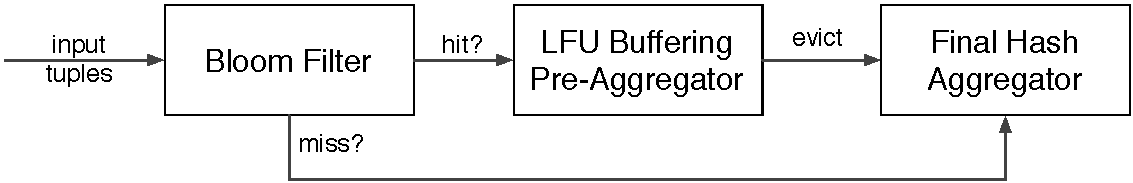
\includegraphics[width=\columnwidth]{figures/aggregator_pipeline}
\end{center}
\caption{An example of an aggregator pipeline}
\label{fig:aggregator_pipeline}
\end{figure}

The techniques described above can be composed into pipelines of aggregators.
Figure~\ref{fig:aggregator_pipeline} shows an example of such a pipeline.
Incoming tuples are routed to a Bloom filter so that the first occurrences of
keys can immediately be sent to the final aggregator, bypassing the
pre-aggregation.  Keys that hit the Bloom filter are sent to a buffering
pre-aggregator.  For now, we'll assume that misses in the pre-aggregation
buffer always cause an existing buffer entry to be evicted (rather than giving
the incoming key a second chance to bypass the pre-aggregator).


Consider the output of this pipeline to be the input to the final hash
aggregator.  Keys appear in this output because either missed the Bloom filter
and bypassed the cache, or were evicted from the cache by other keys.  Let
$d_k(t)$ be the probability that key appears at time $t$:
\[
    d_k(t) = P\left(\text{misses Bloom filter}|t\right)
                +
             P\left(\text{hits BloomFilter}|t\right)
             P\left(\text{not in cache}|t\right)
\]

The probability that a key was evicted from the cache between arrivals can be
calculated from its iterarrival rate in the input stream.  If a key has an
interarrival rate of $n$, then there were $n$ opportunities for it to be
evicted.  If the key remained in the cache, then for every one of those $n$
arrivals either the other keys hit the cache, missed the Bloom filter, or
missed the cache and evicted another key:

\begin{align*}
    P\left(\text{arrival evicts a particular key}\right)
    &=  P\left(\text{misses Bloom filter}\right) + \\
    &
    P\left(\text{hits Bloom filter}\right)
    \left(
        P\left(\text{hits cache}\right)
        + P\left(\text{misses cache}\right)P\left(\text{evicts other key}\right)
    \right)
    \\
\end{align*}

To calculate this, we need to know the overall probabilities of cache hits or
misses.




%%%%%%%%%%%%%%%%%%%%%%%%%%%%%%%%%%%%%%%%%%%%%%%%%%%%%%%%%%%%%%%%%%%%%%%%%%%%%%

\section{Pipelining and Fault-Tolerance}

There are many opportunities for pipelining communication and computation
during aggregation phases, especially when using partial pre-aggregation.
Pipelining makes fault-tolerance more challenging; the most difficult cases
occur when we're pipelining multiple aggregators across different machines.
Simpler cases, such as one-level aggregation with deterministic inputs,
can be made fault-tolerant with simple ``watermark'' schemes.

Most MapReduce-like engines, including Hadoop and Spark, persist the inputs to
disk on the mappers.  This enables efficient recovery of failed reducers,
since they can simply restart and have their inputs replayed.  The cost of
restarting a reducer can be lessened by taking periodic checkpoints of its
state.  Google's XXX system does this by storing reducer state in BigTable.

With barriers between the map and reduce phases (i.e. no pipelining), we don't
have to worry about partial mapper failure; mappers produce their complete
inputs before reducers fetch them.  \textbf{TODO: explain}



\subsection{Deterministic One-level Aggregation}

If we assume that the input to any aggregator is persisted somewhere (or can
be deterministically reconstructed from lineage, as in Spark), then the
machine-local portion of the pre-communication aggregation pipeline can be
made deterministic by re-using the same random number generator seeds.
If a sender crashes while a receiver has processed a portion of its stream,
the receiver can use a ``watermark'' to determine which portions of the
replayed stream can be ignored because they've already been received and
processed.

\subsection{Multi-level Aggregation}

The watermark scheme depends on reduce inputs from the same stream arriving in
a deterministic order.  It can be expensive to provide this guarantee when
pipelining tuples across multiple levels of an aggregation hierarchy.  For
example, consider a setting where each machine has four cores with per-core
pre-aggregators that feed into a machine-local aggregator that feeds into the
network.  Even though the core-level aggregation networks produce deterministic
streams, the \emph{interleaving} of those streams at the machine-level
aggregator may be nondeterministic.  The topology may also change
non-deterministically: when parallelizing recovery of failed mappers, a group
of failed tasks that shared a machine-local aggregator may be split across
different machines.

Essentially, the problem is that failed mappers may pollute the state of all
reducers.  We could choose to throw away work, or we could ensure at-most-once
semantics that let us replay only the unfinished portion of the work without
double-counting.

There are a few approaches that could be used:

\begin{itemize}
    \item Enforce a deterministic interleaving of the streams: intermediate
    aggregators could interleave their streams in a statically-determined
    order.  This makes their output deterministic, but synchronizes the rates
    of their input producers, which may make the job prone to stragglers.

    \item Use a buffering and flushing policy that enables watermarks:
    if intermediate aggregators batched their outputs, they could embed
    watermark vectors in their output that measure progress through their
    inputs.  This requires that messages from a particular input stream
    are incorporated into the output stream in-order to ensure that the
    watermarks are monotonic and strictly increasing.

    \item Use a scheme like Flux to keep multiple synchronized copies of the
    intermediate aggregators.

\end{itemize}


\bibliographystyle{plain}
\bibliography{aggregation}

\end{document}
